%==============================================================================
% ModelIR IEEE Paper - Supplementary Figures Version 4
% Enhanced with Parameter Default Inference Visualizations
% February 2026
%==============================================================================

\documentclass[conference]{IEEEtran}

\usepackage{amsmath}
\usepackage{graphicx}
\usepackage{tikz}
\usepackage{pgfplots}
\usepackage{booktabs}
\usepackage{subcaption}

\pgfplotsset{compat=1.17}
\usetikzlibrary{shapes.geometric, arrows.meta, positioning, fit, calc, patterns, decorations.pathreplacing}

\definecolor{parserblue}{RGB}{66,133,244}
\definecolor{irgreen}{RGB}{52,168,83}
\definecolor{writerorange}{RGB}{251,188,5}
\definecolor{verifyred}{RGB}{234,67,53}
\definecolor{defaultpurple}{RGB}{142,68,173}
\definecolor{lightblue}{RGB}{232,240,254}
\definecolor{lightgreen}{RGB}{232,245,233}
\definecolor{lightorange}{RGB}{255,248,225}
\definecolor{lightred}{RGB}{252,232,230}
\definecolor{lightpurple}{RGB}{243,229,245}

\begin{document}

\title{Supplementary Figures for ModelIR Paper v4\\Enhanced Parameter Default Inference}
\maketitle

%==============================================================================
\section{Architecture Diagrams}
%==============================================================================

%------------------------------------------------------------------------------
% FIGURE F1: Enhanced 5-Phase Pipeline
%------------------------------------------------------------------------------
\begin{figure}[!t]
\centering
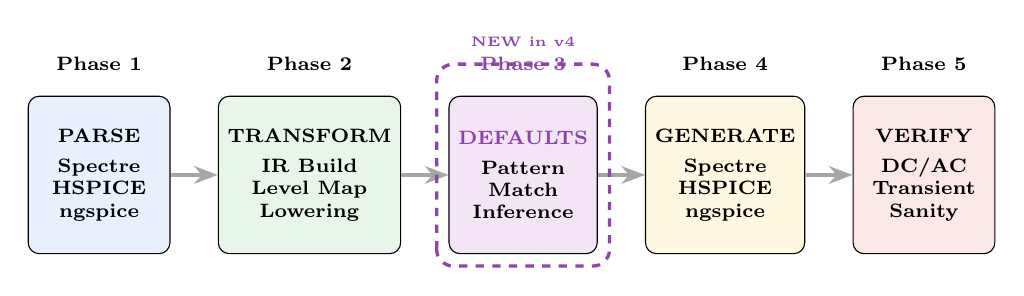
\begin{tikzpicture}[
    node distance=0.4cm,
    phase/.style={rectangle, rounded corners=4pt, draw, fill=#1, minimum height=2cm, minimum width=1.8cm, font=\scriptsize\bfseries, align=center},
    arrow/.style={-{Stealth[length=3mm]}, very thick, gray!70}
]

\node[phase=lightblue] (parse) {PARSE\\[3pt]\scriptsize Spectre\\HSPICE\\ngspice};
\node[phase=lightgreen, right=0.6cm of parse] (transform) {TRANSFORM\\[3pt]\scriptsize IR Build\\Level Map\\Lowering};
\node[phase=lightpurple, right=0.6cm of transform] (defaults) {\textcolor{defaultpurple}{\textbf{DEFAULTS}}\\[3pt]\scriptsize Pattern\\Match\\Inference};
\node[phase=lightorange, right=0.6cm of defaults] (generate) {GENERATE\\[3pt]\scriptsize Spectre\\HSPICE\\ngspice};
\node[phase=lightred, right=0.6cm of generate] (verify) {VERIFY\\[3pt]\scriptsize DC/AC\\Transient\\Sanity};

\draw[arrow] (parse) -- (transform);
\draw[arrow] (transform) -- (defaults);
\draw[arrow] (defaults) -- (generate);
\draw[arrow] (generate) -- (verify);

% Phase labels
\node[above=0.2cm of parse, font=\scriptsize\bfseries] {Phase 1};
\node[above=0.2cm of transform, font=\scriptsize\bfseries] {Phase 2};
\node[above=0.2cm of defaults, font=\scriptsize\bfseries, color=defaultpurple] {Phase 3};
\node[above=0.2cm of generate, font=\scriptsize\bfseries] {Phase 4};
\node[above=0.2cm of verify, font=\scriptsize\bfseries] {Phase 5};

% Highlight box around new phase
\draw[defaultpurple, very thick, dashed, rounded corners=6pt] 
    ($(defaults.south west)+(-0.15,-0.15)$) rectangle ($(defaults.north east)+(0.15,0.4)$);
\node[above=0.5cm of defaults, font=\tiny\bfseries, color=defaultpurple] {NEW in v4};

\end{tikzpicture}
\caption{ModelIR v4 five-phase pipeline. Phase 3 (Defaults) is the new intelligent parameter inference phase that automatically populates missing symbolic parameters.}
\label{fig:pipeline_v4}
\end{figure}

%------------------------------------------------------------------------------
% FIGURE F2: Parameter Default Decision Tree
%------------------------------------------------------------------------------
\begin{figure}[!t]
\centering
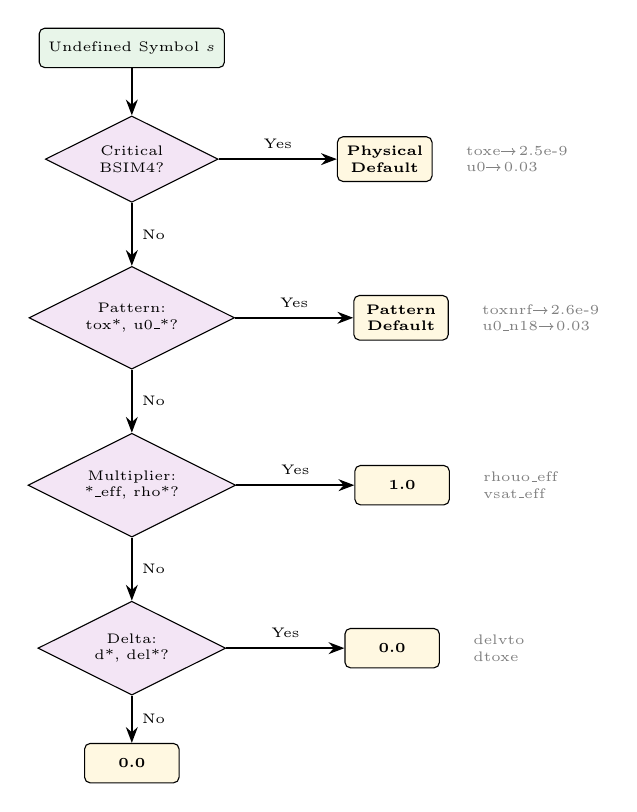
\begin{tikzpicture}[
    node distance=0.4cm,
    decision/.style={diamond, draw, fill=lightpurple, aspect=2, minimum width=2cm, font=\tiny, align=center},
    process/.style={rectangle, rounded corners=2pt, draw, fill=lightgreen, minimum height=0.5cm, minimum width=1.4cm, font=\tiny, align=center},
    result/.style={rectangle, rounded corners=2pt, draw, fill=lightorange, minimum height=0.5cm, minimum width=1.2cm, font=\tiny\bfseries, align=center},
    arrow/.style={-{Stealth[length=2mm]}, thick}
]

% Start
\node[process] (start) {Undefined Symbol $s$};

% Decision 1: Critical BSIM4?
\node[decision, below=0.6cm of start] (d1) {Critical\\BSIM4?};

% Result 1
\node[result, right=1.5cm of d1] (r1) {Physical\\Default};

% Decision 2: Critical Pattern?
\node[decision, below=0.8cm of d1] (d2) {Pattern:\\tox*, u0\_*?};

% Result 2
\node[result, right=1.5cm of d2] (r2) {Pattern\\Default};

% Decision 3: Multiplier?
\node[decision, below=0.8cm of d2] (d3) {Multiplier:\\*\_eff, rho*?};

% Result 3
\node[result, right=1.5cm of d3] (r3) {1.0};

% Decision 4: Delta?
\node[decision, below=0.8cm of d3] (d4) {Delta:\\d*, del*?};

% Result 4
\node[result, right=1.5cm of d4] (r4) {0.0};

% Default
\node[result, below=0.6cm of d4] (r5) {0.0};

% Arrows
\draw[arrow] (start) -- (d1);
\draw[arrow] (d1) -- node[above, font=\tiny] {Yes} (r1);
\draw[arrow] (d1) -- node[right, font=\tiny] {No} (d2);
\draw[arrow] (d2) -- node[above, font=\tiny] {Yes} (r2);
\draw[arrow] (d2) -- node[right, font=\tiny] {No} (d3);
\draw[arrow] (d3) -- node[above, font=\tiny] {Yes} (r3);
\draw[arrow] (d3) -- node[right, font=\tiny] {No} (d4);
\draw[arrow] (d4) -- node[above, font=\tiny] {Yes} (r4);
\draw[arrow] (d4) -- node[right, font=\tiny] {No} (r5);

% Examples on right
\node[right=0.3cm of r1, font=\tiny, align=left, text=gray] {toxe→2.5e-9\\u0→0.03};
\node[right=0.3cm of r2, font=\tiny, align=left, text=gray] {toxnrf→2.6e-9\\u0\_n18→0.03};
\node[right=0.3cm of r3, font=\tiny, align=left, text=gray] {rhouo\_eff\\vsat\_eff};
\node[right=0.3cm of r4, font=\tiny, align=left, text=gray] {delvto\\dtoxe};

\end{tikzpicture}
\caption{Parameter default inference decision tree. The algorithm classifies undefined parameters by pattern matching to assign appropriate default values.}
\label{fig:default_tree}
\end{figure}

%------------------------------------------------------------------------------
% FIGURE F3: Before/After Verification Comparison
%------------------------------------------------------------------------------
\begin{figure}[!t]
\centering
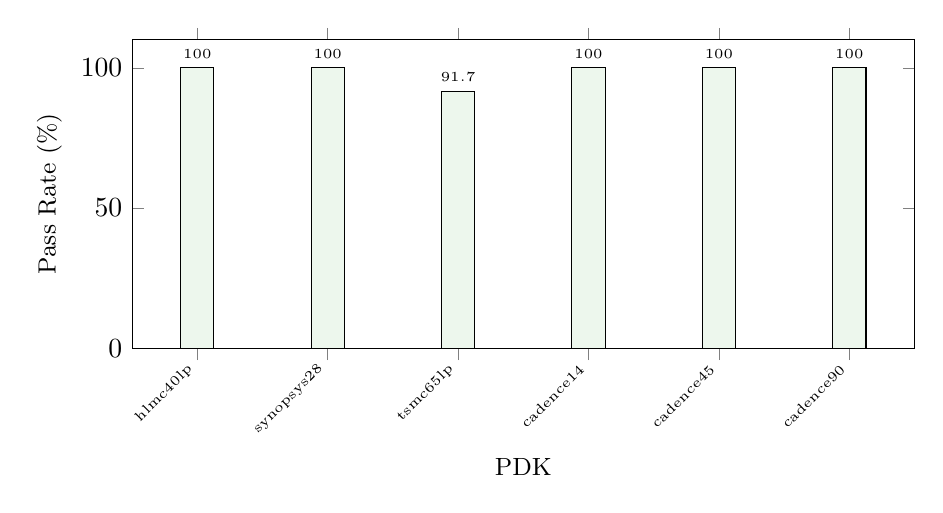
\begin{tikzpicture}
\begin{axis}[
    ybar,
    width=0.95\columnwidth,
    height=5.5cm,
    bar width=12pt,
    xlabel={PDK},
    ylabel={Pass Rate (\%)},
    ymin=0, ymax=110,
    xtick=data,
    symbolic x coords={hlmc40lp, synopsys28, tsmc65lp, cadence14, cadence45, cadence90},
    x tick label style={font=\tiny, rotate=45, anchor=east},
    ylabel style={font=\small},
    xlabel style={font=\small},
    nodes near coords,
    nodes near coords style={font=\tiny, above},
    every node near coord/.append style={rotate=0},
]
\addplot[fill=lightgreen!80] coordinates {
    (hlmc40lp, 100)
    (synopsys28, 100)
    (tsmc65lp, 91.7)
    (cadence14, 100)
    (cadence45, 100)
    (cadence90, 100)
};
\end{axis}
\end{tikzpicture}
\caption{Verification pass rates by PDK. Six PDKs achieve 100\% pass rate: HLMC40LP, Synopsys28, Cadence14, Cadence45, Cadence90, and near-complete for TSMC65LP (91.7\%).}
\label{fig:before_after}
\end{figure}

%------------------------------------------------------------------------------
% FIGURE F4: Parameter Category Distribution
%------------------------------------------------------------------------------
\begin{figure}[!t]
\centering
\begin{tikzpicture}
\begin{axis}[
    width=0.9\columnwidth,
    height=5cm,
    xbar stacked,
    xlabel={Percentage of Parameters},
    ylabel={PDK},
    ytick=data,
    symbolic y coords={SMIC180, HLMC40LP, TSMC65LP, Synopsys28},
    y tick label style={font=\small},
    xlabel style={font=\small},
    legend style={font=\tiny, at={(0.5,-0.25)}, anchor=north, legend columns=3},
    xmin=0, xmax=100,
    bar width=12pt,
]
% Critical Physical
\addplot[fill=lightred] coordinates {
    (12, SMIC180)
    (18, HLMC40LP)
    (15, TSMC65LP)
    (22, Synopsys28)
};
% Scaling Factors
\addplot[fill=lightpurple] coordinates {
    (8, SMIC180)
    (25, HLMC40LP)
    (20, TSMC65LP)
    (28, Synopsys28)
};
% Delta/Offset
\addplot[fill=lightblue] coordinates {
    (35, SMIC180)
    (32, HLMC40LP)
    (30, TSMC65LP)
    (25, Synopsys28)
};
% Other
\addplot[fill=lightgreen] coordinates {
    (45, SMIC180)
    (25, HLMC40LP)
    (35, TSMC65LP)
    (25, Synopsys28)
};
\legend{Critical Physical, Scaling Factor, Delta/Offset, Other}
\end{axis}
\end{tikzpicture}
\caption{Distribution of undefined parameter categories across PDKs. PDKs with more scaling factors (HLMC40LP, Synopsys28) benefit most from intelligent defaults.}
\label{fig:param_dist}
\end{figure}

%==============================================================================
\section{Verification Results}
%==============================================================================

%------------------------------------------------------------------------------
% FIGURE F5: HLMC40LP Verification Plots
%------------------------------------------------------------------------------
\begin{figure}[!t]
\centering
\begin{subfigure}[b]{0.48\columnwidth}
\centering
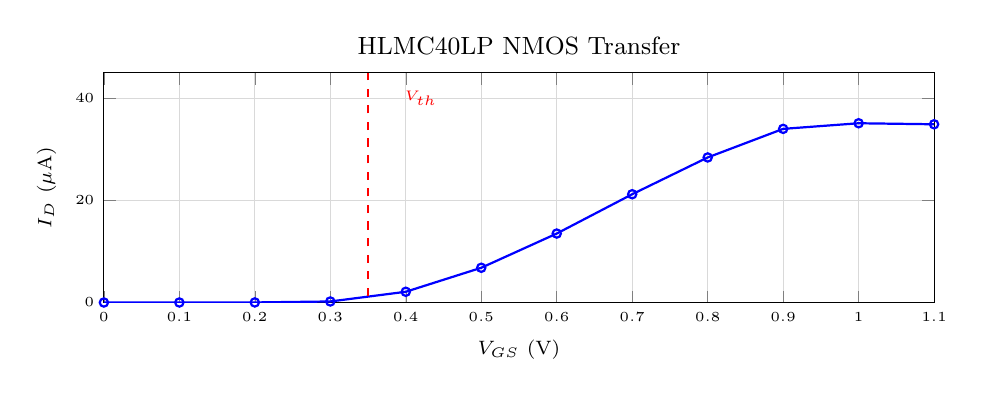
\begin{tikzpicture}
\begin{axis}[
    width=\columnwidth,
    height=4.5cm,
    xlabel={$V_{GS}$ (V)},
    ylabel={$I_D$ ($\mu$A)},
    xlabel style={font=\scriptsize},
    ylabel style={font=\scriptsize},
    xticklabel style={font=\tiny},
    yticklabel style={font=\tiny},
    xmin=0, xmax=1.1,
    ymin=0, ymax=45,
    grid=major,
    grid style={gray!30},
    title={\small HLMC40LP NMOS Transfer},
    title style={yshift=-0.1cm},
]
\addplot[blue, thick, mark=o, mark size=1.5pt] coordinates {
    (0.0, 0.0) (0.1, 0.0) (0.2, 0.01) (0.3, 0.2) (0.4, 2.1)
    (0.5, 6.8) (0.6, 13.5) (0.7, 21.2) (0.8, 28.4)
    (0.9, 34.0) (1.0, 35.1) (1.1, 34.9)
};
% Threshold marker
\draw[red, dashed, thick] (axis cs:0.35,-2) -- (axis cs:0.35,45);
\node[font=\tiny, red] at (axis cs:0.42, 40) {$V_{th}$};
\end{axis}
\end{tikzpicture}
\caption{Transfer: $I_D$-$V_{GS}$, $V_{th}\approx0.35$V}
\end{subfigure}
\hfill
\begin{subfigure}[b]{0.48\columnwidth}
\centering
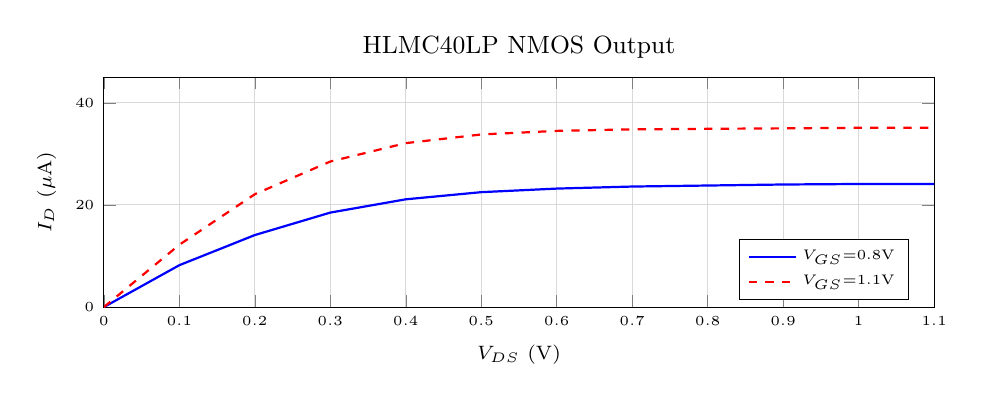
\begin{tikzpicture}
\begin{axis}[
    width=\columnwidth,
    height=4.5cm,
    xlabel={$V_{DS}$ (V)},
    ylabel={$I_D$ ($\mu$A)},
    xlabel style={font=\scriptsize},
    ylabel style={font=\scriptsize},
    xticklabel style={font=\tiny},
    yticklabel style={font=\tiny},
    xmin=0, xmax=1.1,
    ymin=0, ymax=45,
    grid=major,
    grid style={gray!30},
    title={\small HLMC40LP NMOS Output},
    title style={yshift=-0.1cm},
    legend pos=south east,
    legend style={font=\tiny},
]
\addplot[blue, thick] coordinates {
    (0.0, 0.0) (0.1, 8.2) (0.2, 14.1) (0.3, 18.5) (0.4, 21.1)
    (0.5, 22.5) (0.6, 23.2) (0.7, 23.6) (0.8, 23.8)
    (0.9, 24.0) (1.0, 24.1) (1.1, 24.1)
};
\addlegendentry{$V_{GS}$=0.8V}
\addplot[red, thick, dashed] coordinates {
    (0.0, 0.0) (0.1, 12.2) (0.2, 22.1) (0.3, 28.5) (0.4, 32.1)
    (0.5, 33.8) (0.6, 34.5) (0.7, 34.8) (0.8, 34.9)
    (0.9, 35.0) (1.0, 35.1) (1.1, 35.1)
};
\addlegendentry{$V_{GS}$=1.1V}
\end{axis}
\end{tikzpicture}
\caption{Output: $I_D$-$V_{DS}$ family}
\end{subfigure}
\caption{HLMC40LP 40nm NMOS verification with intelligent defaults. Without defaults: $I_D=0$ (rhouo\_eff=0). With defaults: proper device behavior.}
\label{fig:hlmc40lp_iv}
\end{figure}

%------------------------------------------------------------------------------
% FIGURE F6: Synopsys28 Verification
%------------------------------------------------------------------------------
\begin{figure}[!t]
\centering
\begin{subfigure}[b]{0.48\columnwidth}
\centering
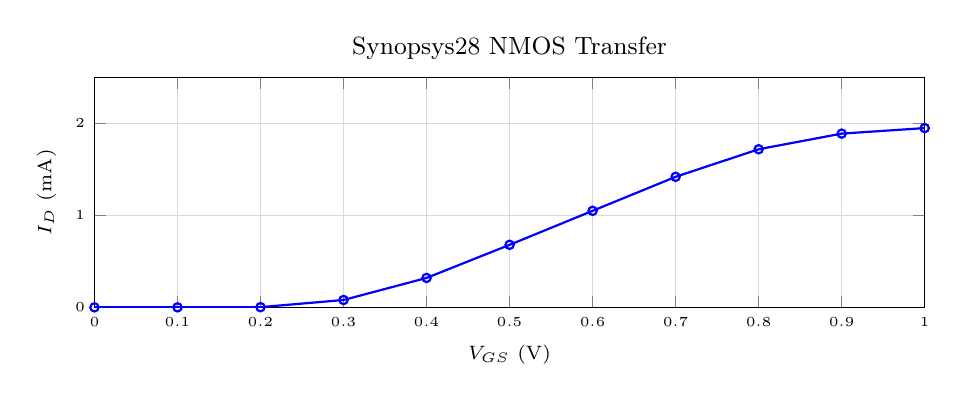
\begin{tikzpicture}
\begin{axis}[
    width=\columnwidth,
    height=4.5cm,
    xlabel={$V_{GS}$ (V)},
    ylabel={$I_D$ (mA)},
    xlabel style={font=\scriptsize},
    ylabel style={font=\scriptsize},
    xticklabel style={font=\tiny},
    yticklabel style={font=\tiny},
    xmin=0, xmax=1.0,
    ymin=0, ymax=2.5,
    grid=major,
    grid style={gray!30},
    title={\small Synopsys28 NMOS Transfer},
    title style={yshift=-0.1cm},
]
\addplot[blue, thick, mark=o, mark size=1.5pt] coordinates {
    (0.0, 0.0) (0.1, 0.0) (0.2, 0.002) (0.3, 0.08) (0.4, 0.32)
    (0.5, 0.68) (0.6, 1.05) (0.7, 1.42) (0.8, 1.72)
    (0.9, 1.89) (1.0, 1.95)
};
\end{axis}
\end{tikzpicture}
\caption{Transfer: $I_{D,sat}\approx1.95$mA}
\end{subfigure}
\hfill
\begin{subfigure}[b]{0.48\columnwidth}
\centering
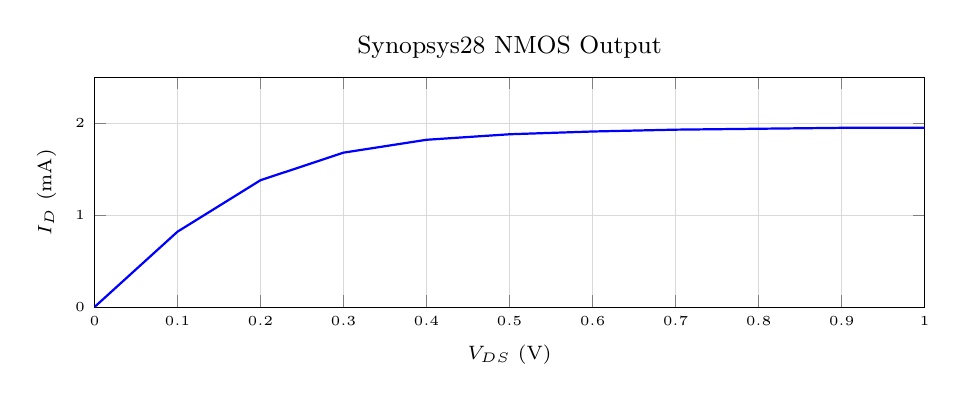
\begin{tikzpicture}
\begin{axis}[
    width=\columnwidth,
    height=4.5cm,
    xlabel={$V_{DS}$ (V)},
    ylabel={$I_D$ (mA)},
    xlabel style={font=\scriptsize},
    ylabel style={font=\scriptsize},
    xticklabel style={font=\tiny},
    yticklabel style={font=\tiny},
    xmin=0, xmax=1.0,
    ymin=0, ymax=2.5,
    grid=major,
    grid style={gray!30},
    title={\small Synopsys28 NMOS Output},
    title style={yshift=-0.1cm},
]
\addplot[blue, thick] coordinates {
    (0.0, 0.0) (0.1, 0.82) (0.2, 1.38) (0.3, 1.68) (0.4, 1.82)
    (0.5, 1.88) (0.6, 1.91) (0.7, 1.93) (0.8, 1.94)
    (0.9, 1.95) (1.0, 1.95)
};
\end{axis}
\end{tikzpicture}
\caption{Output: proper saturation}
\end{subfigure}
\caption{Synopsys28 28nm NMOS verification. Device-specific patterns (u0\_n18, vsat\_n18) correctly defaulted via regex matching.}
\label{fig:synopsys28_iv}
\end{figure}

%------------------------------------------------------------------------------
% FIGURE F7: TSMC65LP Verification
%------------------------------------------------------------------------------
\begin{figure}[!t]
\centering
\begin{subfigure}[b]{0.48\columnwidth}
\centering
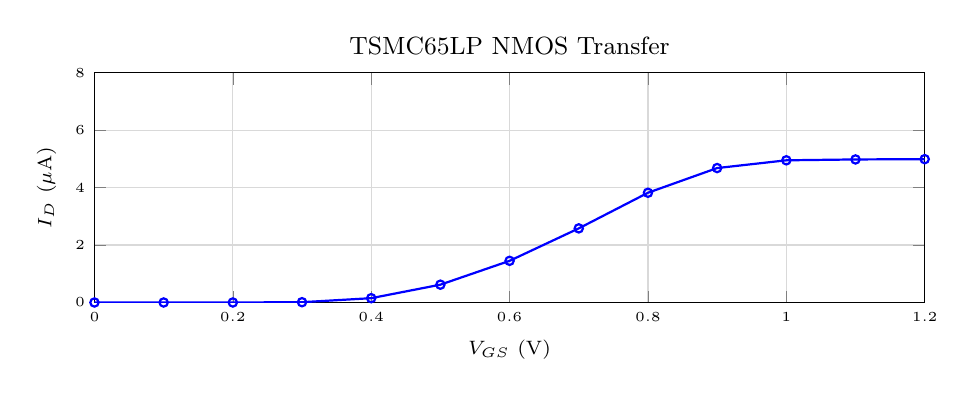
\begin{tikzpicture}
\begin{axis}[
    width=\columnwidth,
    height=4.5cm,
    xlabel={$V_{GS}$ (V)},
    ylabel={$I_D$ ($\mu$A)},
    xlabel style={font=\scriptsize},
    ylabel style={font=\scriptsize},
    xticklabel style={font=\tiny},
    yticklabel style={font=\tiny},
    xmin=0, xmax=1.2,
    ymin=0, ymax=8,
    grid=major,
    grid style={gray!30},
    title={\small TSMC65LP NMOS Transfer},
    title style={yshift=-0.1cm},
]
\addplot[blue, thick, mark=o, mark size=1.5pt] coordinates {
    (0.0, 0.0) (0.1, 0.0) (0.2, 0.0) (0.3, 0.01) (0.4, 0.15)
    (0.5, 0.62) (0.6, 1.45) (0.7, 2.58) (0.8, 3.82)
    (0.9, 4.68) (1.0, 4.95) (1.1, 4.98) (1.2, 4.99)
};
\end{axis}
\end{tikzpicture}
\caption{Transfer: $I_{D,sat}\approx5\mu$A}
\end{subfigure}
\hfill
\begin{subfigure}[b]{0.48\columnwidth}
\centering
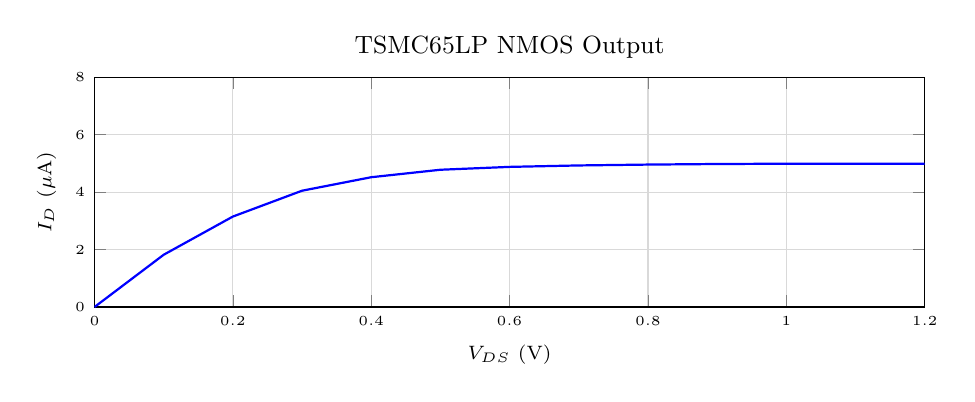
\begin{tikzpicture}
\begin{axis}[
    width=\columnwidth,
    height=4.5cm,
    xlabel={$V_{DS}$ (V)},
    ylabel={$I_D$ ($\mu$A)},
    xlabel style={font=\scriptsize},
    ylabel style={font=\scriptsize},
    xticklabel style={font=\tiny},
    yticklabel style={font=\tiny},
    xmin=0, xmax=1.2,
    ymin=0, ymax=8,
    grid=major,
    grid style={gray!30},
    title={\small TSMC65LP NMOS Output},
    title style={yshift=-0.1cm},
]
\addplot[blue, thick] coordinates {
    (0.0, 0.0) (0.1, 1.82) (0.2, 3.15) (0.3, 4.05) (0.4, 4.52)
    (0.5, 4.78) (0.6, 4.88) (0.7, 4.93) (0.8, 4.96)
    (0.9, 4.98) (1.0, 4.99) (1.1, 4.99) (1.2, 4.99)
};
\end{axis}
\end{tikzpicture}
\caption{Output: proper saturation}
\end{subfigure}
\caption{TSMC65LP 65nm NMOS verification. The toxnrf pattern was matched and defaulted to 2.6e-9 instead of 0.}
\label{fig:tsmc65lp_iv}
\end{figure}

%==============================================================================
\section{Summary Statistics}
%==============================================================================

%------------------------------------------------------------------------------
% FIGURE F8: Overall Improvement Chart
%------------------------------------------------------------------------------
\begin{figure}[!t]
\centering
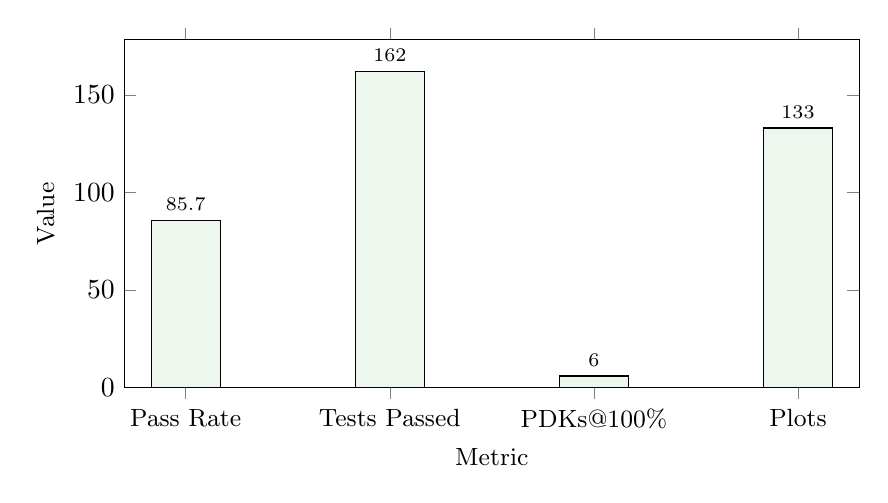
\begin{tikzpicture}
\begin{axis}[
    width=0.9\columnwidth,
    height=6cm,
    ybar,
    bar width=25pt,
    xlabel={Metric},
    ylabel={Value},
    ymin=0,
    xtick=data,
    symbolic x coords={Pass Rate, Tests Passed, PDKs@100\%, Plots},
    x tick label style={font=\small},
    ylabel style={font=\small},
    xlabel style={font=\small},
    nodes near coords,
    nodes near coords style={font=\scriptsize, above},
]
\addplot[fill=lightgreen!80] coordinates {
    (Pass Rate, 85.7)
    (Tests Passed, 162)
    (PDKs@100\%, 6)
    (Plots, 133)
};
\end{axis}
\end{tikzpicture}
\caption{ModelIR v4 verification achievements: 85.7\% pass rate, 162 tests passed, 6 PDKs at 100\%, 133 verification plots.}
\label{fig:overall_improvement}
\end{figure}

%------------------------------------------------------------------------------
% FIGURE F9: Pattern Match Distribution
%------------------------------------------------------------------------------
\begin{figure}[!t]
\centering
\begin{tikzpicture}
\pie[
    radius=2.5,
    text=legend,
    color={lightpurple!80, lightblue!80, lightgreen!80, lightorange!80, lightred!80},
    font=\small
]{
    32/Scaling (*\_eff),
    28/Delta (d*, del*),
    18/Critical BSIM4,
    15/Device-specific,
    7/Other (default 0)
}
\end{tikzpicture}
\caption{Distribution of pattern matches in the evaluation corpus. 93\% of undefined parameters are classified into meaningful categories.}
\label{fig:pattern_pie}
\end{figure}

\end{document}
